\chapter{Architettura a microservizi}\label{ch-06}

\lecturemeta{Capitolo originale: 6 --- Microservices Architecture \quad\textbullet\quad Antonio Brogi}{Appunti di Emiliano Sescu (github.com/Faxatos), cap. 6}

Questo capitolo tratta le \textbf{architetture a microservizi}: idee di
base, principi e vantaggi che le rendono così diffuse. Partiamo da una
domanda: \textbf{come si divide un sistema in componenti?}

Dividere il sistema in componenti è il primo passo per adottare i
microservizi. I motivi per farlo sono diversi:

\begin{itemize}
\tightlist
\item
  team diversi possono lavorare \textbf{in parallelo};
\item
  favorisce il \textbf{riuso};
\item
  rende più facile \textbf{distribuire} il sistema su più computer;
\item
  permette di replicare, eseguire in parallelo e spostare i componenti,
  sfruttando al massimo le capacità del cloud (scalabilità,
  affidabilità, flessibilità).
\end{itemize}

Tra i principi dei microservizi è centrale l'uso di \textbf{servizi
senza stato} (\emph{stateless}), che salvano le informazioni persistenti
in \textbf{database locali}. Questo rende il sistema agile e scalabile
(i servizi si possono spostare tra server virtuali quando serve) e aiuta
a costruire sistemi resilienti e tolleranti ai guasti.

\begin{boxdefinition}{Servizio software}

Un \textbf{servizio software} è un componente software accessibile via
Internet. Si usa tramite la sua \textbf{interfaccia pubblica}, che
nasconde tutti i dettagli di implementazione. Dato un input, produce
l'output corrispondente \textbf{senza effetti collaterali}.

\end{boxdefinition}

I servizi \textbf{non mantengono uno stato interno}: lo stato è salvato
in un database esplicito oppure lo conserva chi chiama il servizio.
Quando serve uno stato, la richiesta contiene lo stato e la risposta
contiene il risultato insieme allo stato aggiornato.

Un po' di storia che ha portato ai microservizi:

\begin{itemize}
\tightlist
\item
  \textbf{Service-Oriented Architecture} (SOA, fine anni '90):
  applicazioni fatte di tanti blocchi, ognuno una classe o un oggetto. I
  blocchi erano indipendenti e potevano essere scritti con tecnologie
  diverse, perché comunicavano tra loro (o con Internet) tramite
  interfacce pubbliche.
\item
  \textbf{Web Services} (primi anni 2000): servizi basati su standard
  (XML, SOAP, WSDL e molti altri), usati per descrivere i servizi
  (input, output, tipi dei parametri, \ldots). Gli standard erano utili,
  ma erano così tanti da diventare difficili da gestire.
\item
  \textbf{Sistemi a servizi moderni} (oggi): protocolli di interazione e
  interfacce molto più semplici, con formati più efficienti per
  codificare i messaggi. Risultato: meno overhead ed esecuzione più
  veloce.
\end{itemize}

\textbf{Amazon Web Services} ha avuto un grande impatto su questo mondo,
con un ``manifesto'' di linee guida su come implementare i servizi:

\begin{itemize}
\tightlist
\item
  un servizio deve riguardare \textbf{una sola funzione di business};
\item
  i servizi devono essere \textbf{completamente indipendenti}, ognuno
  con il \textbf{proprio database};
\item
  un servizio deve gestire la \textbf{propria interfaccia utente};
\item
  deve essere possibile sostituire o replicare un servizio \textbf{senza
  cambiare gli altri}.
\end{itemize}

Da qui nascono i \textbf{microservizi}: servizi in genere piccoli, senza
stato e con \textbf{una sola responsabilità}.

\begin{figure}[H]
\centering
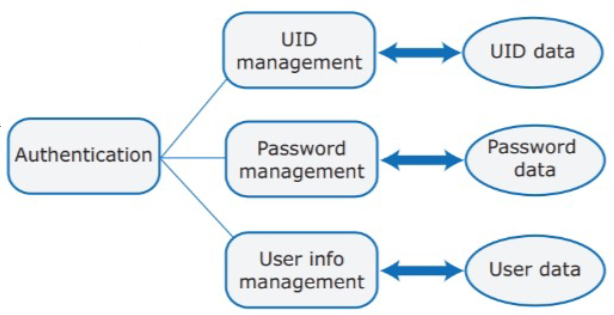
\includegraphics[width=0.70\linewidth,height=0.45\textheight,keepaspectratio]{images/06-microservizi_fig6-1_autenticazione.png}
\caption{Esempio di sistema che usa un modulo di autenticazione.}
\end{figure}

\begin{boxexample}{Dividere un modulo di autenticazione}

Prendiamo un sistema con un modulo di autenticazione che offre:
registrazione, autenticazione con UID/password, autenticazione a due
fattori, gestione delle informazioni utente, reset della password. La
Fig. 6.1 mostra una possibile divisione in microservizi.

Per trovare i microservizi si spezzano le feature ``grosse'' in funzioni
più dettagliate, si guardano i dati usati e si crea \textbf{un
microservizio per ogni dato logico da gestire} (ogni servizio ha i
propri dati). Se un servizio ha bisogno dei dati di un altro, li chiede
tramite interfaccia oppure replica solo alcuni dati critici (accettando
problemi di consistenza), cercando di replicare il meno possibile.

\end{boxexample}

\section{Microservizi}\label{microservizi}

\begin{boxdefinition}{Microservizio}

Un \textbf{microservizio} è un servizio \textbf{indipendente} (la sua
interfaccia non è toccata dai cambiamenti degli altri servizi) e di
solito \textbf{piccolo}, che si combina con altri per creare
applicazioni. Deve essere possibile modificarlo e ripubblicarlo
\textbf{senza cambiare o fermare gli altri servizi}.

\end{boxdefinition}

Caratteristiche che un microservizio deve avere:

\begin{itemize}
\tightlist
\item
  \textbf{Autonomo} (\emph{self-contained}): poche dipendenze esterne.
  Gestisce i propri dati e la propria interfaccia utente, quindi si può
  installare e cambiare subito.
\item
  \textbf{Leggero} (\emph{lightweight}): comunica con protocolli
  leggeri, così l'overhead di comunicazione è basso.
\item
  \textbf{Indipendente dall'implementazione}: ogni microservizio può
  essere scritto in un linguaggio diverso e usare tecnologie diverse.
\item
  \textbf{Installabile da solo} (\emph{independently deployable}): ogni
  microservizio gira nel suo processo e si installa in modo indipendente
  con sistemi automatici.
\item
  \textbf{Orientato al business}: deve implementare capacità e bisogni
  di business, non solo offrire un servizio tecnico. Questo si sposa
  bene con i framework Agile.
\end{itemize}

Due misure importanti per i microservizi sono:

\begin{itemize}
\tightlist
\item
  l'\textbf{accoppiamento} (\emph{coupling}): quante relazioni ci sono
  \textbf{tra} componenti diversi;
\item
  la \textbf{coesione} (\emph{cohesion}): quante relazioni ci sono
  \textbf{dentro} un componente.
\end{itemize}

L'obiettivo è \textbf{basso accoppiamento e alta coesione}: basso
accoppiamento vuol dire servizi e aggiornamenti indipendenti, alta
coesione vuol dire meno comunicazione (e quindi meno overhead) tra
servizi.

\begin{boxtip}{Quanto deve essere grande un microservizio?}

Ogni servizio deve fare \textbf{una sola cosa, e farla bene}
(\emph{Single Responsibility Principle}). Per le dimensioni si usa la
\textbf{regola del due}: un servizio deve poter essere sviluppato,
testato e installato da un team in \textbf{due settimane}, e il team
deve poter essere sfamato con \textbf{due pizze grandi} (8-10 persone).

\end{boxtip}

Servono così tante persone perché il team deve: implementare le
funzionalità del servizio; scrivere il codice che lo rende completamente
indipendente; elaborare i messaggi in entrata e in uscita; gestire i
guasti (ci saranno quasi sicuramente guasti dei servizi e delle
interazioni); gestire la consistenza dei dati usati anche da altri
servizi (problema serio quando i dati sono replicati); mantenere
l'interfaccia del servizio; testare il servizio e le sue interazioni;
supportare il servizio dopo il rilascio (\textbf{``you build it, you run
it''}, chi lo costruisce lo gestisce).

Anni fa c'erano team diversi per lo sviluppo e per la produzione; oggi
si usa molto il \textbf{DevOps}, in cui le stesse persone costruiscono e
mantengono il servizio.

\section{Architettura}\label{architettura}

Le due motivazioni principali per usare un'architettura a microservizi
sono:

\begin{itemize}
\tightlist
\item
  \textbf{ridurre i tempi} per rilasciare nuove feature e aggiornamenti;
\item
  \textbf{scalare}.
\end{itemize}

Mettendo i microservizi in container separati, ognuno si può fermare e
riavviare velocemente senza toccare gli altri, e le repliche si possono
installare in fretta. Se questi due aspetti sono importanti per
l'applicazione, i microservizi sono la scelta giusta; altrimenti (per
un'applicazione semplice) un'\textbf{applicazione monolitica} va
benissimo.

\begin{figure}[H]
\centering
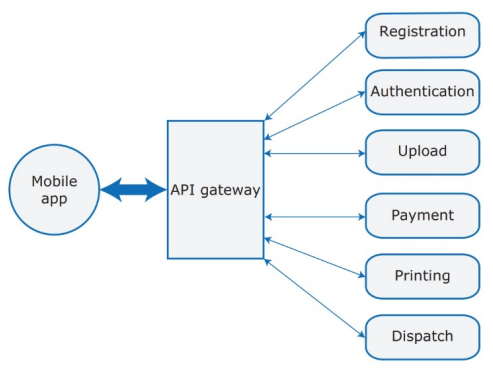
\includegraphics[width=0.65\linewidth,height=0.45\textheight,keepaspectratio]{images/06-microservizi_fig6-2_stampa-foto.png}
\caption{Sistema di stampa foto per dispositivi mobili.}
\end{figure}

La Fig. 6.2 mostra che i microservizi aiutano a individuare i servizi di
base dell'applicazione: c'è un servizio separato per ogni area di
funzionalità. Mostra anche una buona pratica: usare un \textbf{API
gateway} come unico punto di contatto tra l'app mobile e i microservizi.
È il gateway a inoltrare ogni richiesta al microservizio giusto.

Nelle architetture a microservizi bisogna prendere \textbf{cinque
decisioni di design}:

\begin{enumerate}
\def\labelenumi{\arabic{enumi}.}
\tightlist
\item
  Quali microservizi compongono il sistema?
\item
  Come comunicano tra loro?
\item
  Come si distribuiscono e condividono i dati?
\item
  Come si coordinano i microservizi?
\item
  Come si rilevano, segnalano e gestiscono i guasti?
\end{enumerate}

Le vediamo una per una.

\subsection{Decomposizione del
sistema}\label{decomposizione-del-sistema}

La decomposizione è una delle scelte più importanti, ma anche delle più
difficili. Con \textbf{troppi} microservizi, funzionalità collegate
finiscono in servizi diversi che devono parlarsi di continuo: tanta
comunicazione, quindi molto overhead. Con \textbf{troppo pochi}, ogni
servizio fa troppe cose e i servizi diventano poco indipendenti negli
aggiornamenti e nel deploy. Alcuni consigli:

\begin{itemize}
\tightlist
\item
  trovare il giusto equilibrio tra funzionalità molto fini e prestazioni
  del sistema;
\item
  seguire il \textbf{common closure principle}: gli elementi che
  probabilmente cambieranno insieme devono stare nello stesso servizio;
\item
  associare i servizi alle \textbf{capacità di business};
\item
  ogni servizio deve accedere \textbf{solo ai dati che gli servono} (con
  meccanismi per propagare i dati quando serve).
\end{itemize}

\begin{boxtip}{Da dove partire}

Ragionare direttamente a microservizi è difficile: per questo si parte
spesso da un \textbf{monolite} e lo si divide in seguito. Un buon modo
per capire come dividere è guardare i \textbf{dati} che i servizi devono
gestire.

\end{boxtip}

\subsection{Comunicazione tra servizi}\label{comunicazione-tra-servizi}

La seconda scelta riguarda come comunicano i servizi.

\begin{figure}[H]
\centering
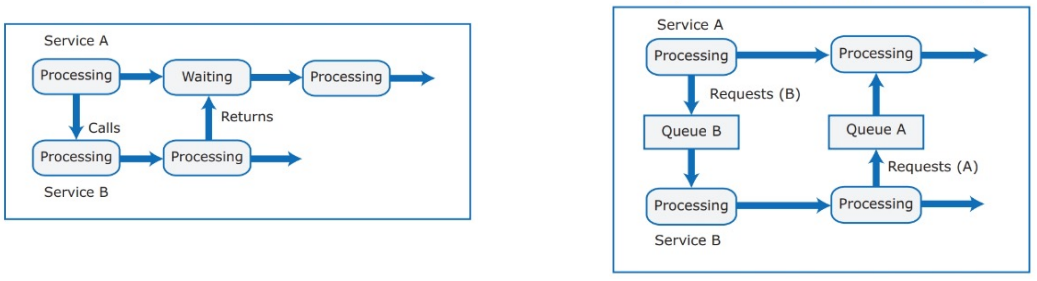
\includegraphics[width=1.00\linewidth,height=0.45\textheight,keepaspectratio]{images/06-microservizi_fig6-3_sincrona-asincrona.png}
\caption{Interazione sincrona e asincrona tra servizi.}
\end{figure}

La prima scelta (Fig. 6.3) è tra comunicazione \textbf{sincrona} e
\textbf{asincrona}:

\begin{itemize}
\tightlist
\item
  la \textbf{sincrona} (a sinistra) è più facile da scrivere e da
  capire;
\item
  l'\textbf{asincrona} (a destra) ha un accoppiamento più basso ed è più
  efficiente, ma è più difficile da scrivere (serve una coda per le
  richieste) e da capire.
\end{itemize}

\begin{figure}[H]
\centering
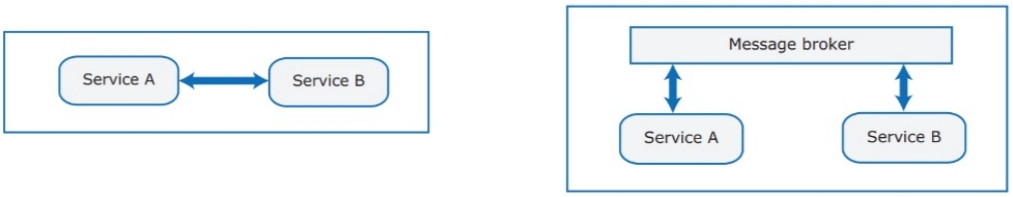
\includegraphics[width=1.00\linewidth,height=0.45\textheight,keepaspectratio]{images/06-microservizi_fig6-4_diretta-indiretta.png}
\caption{Comunicazione diretta e indiretta tra servizi.}
\end{figure}

La seconda scelta (Fig. 6.4) è tra comunicazione \textbf{diretta} e
\textbf{indiretta}:

\begin{itemize}
\tightlist
\item
  nella \textbf{diretta} un servizio manda messaggi direttamente a un
  altro. È più semplice e veloce, ma chi chiama deve conoscere gli URI
  degli altri servizi;
\item
  nella \textbf{indiretta} si usa un \textbf{message broker} (o una
  coda) che trova l'indirizzo del servizio richiesto e si occupa di
  tradurre i messaggi. Supporta sia interazioni sincrone sia asincrone e
  rende più facile modificare e sostituire i servizi, ma è più complessa
  e lenta.
\end{itemize}

\subsection{Distribuzione e condivisione dei
dati}\label{distribuzione-e-condivisione-dei-dati}

Ogni microservizio deve \textbf{gestire i propri dati}, perché vogliamo
che i microservizi siano indipendenti (gli altri non devono sapere come
sono organizzati i suoi dati). Ci saranno comunque dipendenze tra i dati
di servizi diversi. Per gestirle:

\begin{itemize}
\tightlist
\item
  condividere \textbf{il meno possibile};
\item
  condividere \textbf{in sola lettura}, con pochi servizi responsabili
  degli aggiornamenti;
\item
  prevedere un meccanismo per tenere \textbf{consistenti} le copie del
  database usate dai servizi replicati.
\end{itemize}

Un meccanismo classico per la consistenza sono le \textbf{transazioni
ACID} (\emph{Atomicity, Consistency, Isolation, Durability}): gli
aggiornamenti vengono serializzati, cioè il database passa da uno stato
consistente a un altro, evitando inconsistenze. Nei sistemi distribuiti
però bisogna scegliere tra consistenza e prestazioni, e con i
microservizi il sistema va progettato per \textbf{tollerare un po' di
inconsistenza}. Ci sono due tipi di inconsistenza da gestire:

\begin{itemize}
\tightlist
\item
  \textbf{Inconsistenza di dati dipendenti}: le azioni o i guasti di un
  servizio possono rendere inconsistenti i dati gestiti da un altro
  servizio.
\item
  \textbf{Inconsistenza tra repliche}: più repliche dello stesso
  servizio girano insieme, ognuna con la propria copia del database che
  aggiorna per conto suo. Le copie devono diventare \textbf{prima o poi}
  consistenti (\emph{eventual consistency}).
\end{itemize}

\subsubsection{Il teorema CAP}\label{il-teorema-cap}

\begin{boxtheorem}{Teorema CAP (congettura di Brewer, PODC 2000)}

È impossibile per un servizio web garantire \textbf{contemporaneamente}:

\begin{itemize}
\tightlist
\item
  \textbf{Consistency} (consistenza): ogni servizio restituisce la
  risposta corretta a ogni richiesta;
\item
  \textbf{Availability} (disponibilità): ogni richiesta prima o poi
  riceve una risposta;
\item
  \textbf{Partition tolerance} (tolleranza alle partizioni): i servizi
  possono essere divisi in più gruppi, e la rete può ritardare o perdere
  quanti messaggi vuole tra i servizi.
\end{itemize}

\end{boxtheorem}

Una riformulazione successiva (Gilbert e Lynch, 2012) dice: \emph{in una
rete soggetta a guasti di comunicazione, è impossibile per qualsiasi
servizio web implementare una memoria condivisa atomica in
lettura/scrittura che garantisca una risposta a ogni richiesta}. In
pratica, visto che le partizioni di rete capitano, bisogna
\textbf{scegliere tra consistenza e disponibilità}.

\begin{boxtip}{Idea della dimostrazione (versione semplificata)}

Siano S1 e S2 due repliche dello stesso servizio in due partizioni di
rete diverse, e supponiamo che ogni messaggio tra S1 e S2 possa essere
ritardato o perso. Un client scrive il valore V1 su S1. Poi un altro
client legge da S2. S2 non può sapere se S1 ha ricevuto una scrittura
(il messaggio potrebbe essersi perso). Allora ha due scelte:

\begin{itemize}
\tightlist
\item
  \textbf{risponde subito} con il valore che ha: la risposta può essere
  vecchia, quindi si perde la \textbf{consistenza};
\item
  \textbf{aspetta} di sentire S1 per essere sicuro: ma il messaggio
  potrebbe non arrivare mai, quindi si perde la \textbf{disponibilità}.
\end{itemize}

\end{boxtip}

Soluzioni pratiche:

\begin{itemize}
\tightlist
\item
  garantire la \textbf{disponibilità} e offrire consistenza ``al meglio
  possibile'' (\emph{best-effort}): è la soluzione più comune;
\item
  garantire la \textbf{consistenza forte} e offrire disponibilità
  best-effort: si usa quando la consistenza è indispensabile (es.
  applicazioni finanziarie);
\item
  trovare un \textbf{compromesso} (es. tollerare dati vecchi di un'ora,
  ma non di un giorno).
\end{itemize}

\subsubsection{Il pattern Saga}\label{il-pattern-saga}

Come si implementano le transazioni distribuite con un pattern?

\begin{boxdefinition}{Saga}

Il \textbf{pattern Saga} implementa ogni transazione di business che
coinvolge più servizi come una \textbf{saga}, cioè una \textbf{sequenza
di transazioni locali} (Fig. 6.5). Ogni transazione locale aggiorna un
database e fa partire la transazione locale successiva. Se una
transazione locale fallisce, la saga esegue una serie di
\textbf{transazioni di compensazione} (invece di fare rollback, che con
i microservizi a volte non è possibile).

\end{boxdefinition}

\begin{figure}[H]
\centering
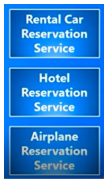
\includegraphics[width=0.19\linewidth,height=0.45\textheight,keepaspectratio]{images/06-microservizi_fig6-5_saga.png}
\caption{Esempio di saga.}
\end{figure}

Le saghe si possono coordinare in due modi:

\begin{itemize}
\tightlist
\item
  \textbf{Coreografia}: ogni transazione locale pubblica degli eventi
  che fanno partire le transazioni successive.
\item
  \textbf{Orchestrazione}: un \textbf{orchestratore} dice ai
  partecipanti quali transazioni locali eseguire.
\end{itemize}

Anche le transazioni di compensazione si possono fare in due modi:

\begin{itemize}
\tightlist
\item
  \textbf{modello backward} (all'indietro): si annullano le modifiche
  fatte dalle transazioni locali già eseguite;
\item
  \textbf{modello forward} (in avanti): si applica il principio
  ``\textbf{riprova più tardi}''.
\end{itemize}

\begin{boxexample}{L'approccio di Netflix}

Netflix replica i dati su \emph{n} nodi con \textbf{Apache Cassandra}
per ottenere la consistenza finale: il sistema prova ad aggiornare più
repliche possibile, e richiede che rispondano almeno
\(\lfloor n/2 \rfloor + 1\) repliche (la maggioranza). È un esempio di
compromesso ottenibile con l'eventual consistency.

\end{boxexample}

\subsection{Coordinamento dei servizi}\label{coordinamento-dei-servizi}

Il coordinamento dei servizi si può fare in due modi:

\begin{itemize}
\tightlist
\item
  \textbf{Orchestrazione}: un orchestratore dice ai microservizi come
  devono ``suonare''.
\item
  \textbf{Coreografia}: i microservizi si gestiscono da soli.
\end{itemize}

\begin{boxtip}{Un'immagine per ricordarlo}

L'orchestrazione è come un \textbf{semaforo} (qualcuno decide per
tutti), la coreografia è come una \textbf{rotonda} (ognuno si regola da
sé seguendo le regole).

\end{boxtip}

\begin{figure}[H]
\centering
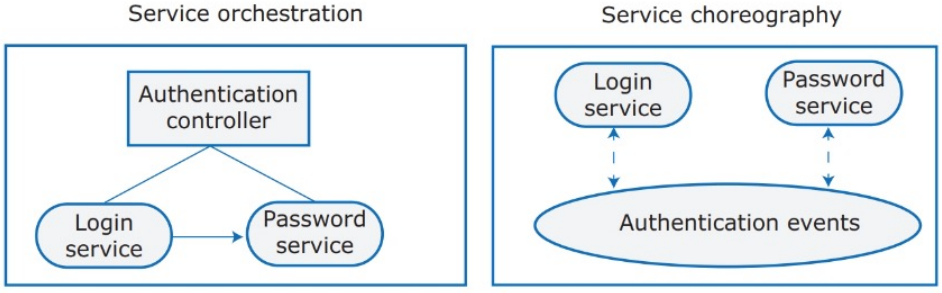
\includegraphics[width=1.00\linewidth,height=0.45\textheight,keepaspectratio]{images/06-microservizi_fig6-6_orchestrazione-coreografia.png}
\caption{Esempio di orchestrazione e coreografia.}
\end{figure}

Nella Fig. 6.6, con l'\textbf{orchestrazione} c'è un controller
esplicito che coordina il sistema (l'\emph{Authentication controller});
con la \textbf{coreografia} si usa una sincronizzazione basata su
\textbf{eventi} (un meccanismo publish \& subscribe chiamato
\emph{Authentication events}). La coreografia evita un controller in più
(che sarebbe un \textbf{single point of failure}), ma è più difficile da
debuggare e da ripristinare in caso di guasto.

\begin{boxtip}{Buona pratica}

Partire sempre con l'\textbf{orchestrazione} (più facile da progettare)
e passare alla coreografia solo se il prodotto diventa rigido o
difficile da aggiornare.

\end{boxtip}

\subsection{Gestione dei guasti}\label{gestione-dei-guasti}

Prima o poi qualcosa andrà storto, inevitabilmente.

\begin{boxexample}{Quanto costa dipendere da altri servizi}

Un servizio offre una funzionalità F chiamando altri due servizi, ognuno
disponibile il 99\% del tempo e indipendenti tra loro. F è disponibile
solo quando lo sono entrambi: \(0{,}99 \times 0{,}99 = 0{,}9801\), cioè
circa il 98\%. Il restante 2\% di un giorno (1440 minuti) sono circa
\textbf{30 minuti al giorno} di non disponibilità.

\end{boxexample}

Soprattutto negli ambienti distribuiti, bisogna gestire i guasti: i
servizi devono essere \textbf{progettati per sopravvivere ai guasti}. Ci
sono tre tipi principali di guasto:

\begin{itemize}
\tightlist
\item
  \textbf{Guasto interno} (\emph{internal service failure}): il servizio
  stesso rileva il problema e può segnalarlo a chi lo ha chiamato con un
  messaggio di errore. Esempio: un servizio riceve un URL in input e
  scopre che il link non è valido.
\item
  \textbf{Guasto esterno} (\emph{external service failure}): una causa
  esterna compromette la disponibilità del servizio, che può smettere di
  rispondere; bisogna intervenire per riavviarlo.
\item
  \textbf{Guasto di prestazioni} (\emph{service performance failure}):
  le prestazioni del servizio scendono sotto un livello accettabile, per
  carico eccessivo o per un problema interno. Un monitoraggio esterno
  può rilevare sia i guasti di prestazioni sia i servizi che non
  rispondono.
\end{itemize}

\subsubsection{Circuit breaker}\label{circuit-breaker}

Una delle soluzioni più tipiche per i microservizi è il \textbf{circuit
breaker} (interruttore automatico): un design pattern che rende i
microservizi resilienti limitando l'impatto di guasti e ritardi dei
servizi.

Funziona così (Fig. 6.7): tra il client e il servizio remoto (il
\emph{supplier}) si aggiunge un componente, il circuit breaker.

\begin{enumerate}
\def\labelenumi{\arabic{enumi}.}
\tightlist
\item
  Il circuit breaker riceve la richiesta dal client, la inoltra al
  servizio remoto e fa partire un timer.
\item
  Se il servizio remoto risponde in tempo, il circuit breaker inoltra la
  risposta al client.
\item
  Se scade il timer (il servizio è guasto o troppo lento), il circuit
  breaker dice al client che il servizio remoto ha fallito, così il
  client non resta bloccato ad aspettare.
\item
  Dopo più fallimenti il circuit breaker \textbf{scatta} (\emph{trip}):
  per un certo periodo tutte le chiamate al servizio remoto falliscono
  \textbf{subito}, senza nemmeno provarci (circuito aperto).
\item
  Finito il periodo, lascia passare un numero limitato di richieste di
  prova. Se vanno a buon fine torna al funzionamento normale, altrimenti
  il periodo di attesa ricomincia.
\end{enumerate}

\begin{figure}[H]
\centering
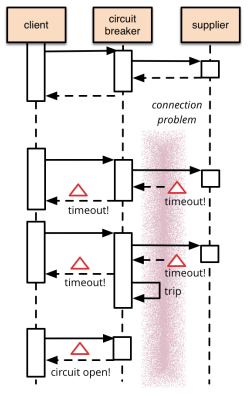
\includegraphics[width=0.40\linewidth,height=0.45\textheight,keepaspectratio]{images/06-microservizi_fig6-7_circuit-breaker.png}
\caption{Esempio di diagramma di sequenza di un circuit breaker.}
\end{figure}

\begin{boxexample}{Il circuit breaker di Spotify}

Il servizio di ricerca di Spotify a volte fallisce (deve cercare in un
indice enorme di canzoni). Allora Spotify ricarica velocemente la pagina
e usa il tempo che l'utente impiega a scrivere il nome della canzone
come periodo di attesa. Nessun messaggio di errore compare all'utente.

\end{boxexample}

Ci sono molti modi per testare la gestione dei guasti. Uno interessante
è \textbf{Chaos Monkey} di Netflix (dal \emph{chaos engineering}): uno
strumento che spegne a caso istanze di VM e container \textbf{in
produzione}. Visto che si fa direttamente in produzione, è un test
``coraggioso''.

\section{Servizi RESTful}\label{servizi-restful}

I microservizi sono \textbf{servizi RESTful}. \textbf{REST}
(\emph{REpresentational State Transfer}) ha quattro principi:

\begin{itemize}
\tightlist
\item
  \textbf{Identificazione delle risorse tramite URI}: il servizio espone
  un insieme di risorse, ognuna identificata da un \textbf{URI}
  (\emph{Uniform Resource Identifier}, una sequenza di caratteri che
  identifica una risorsa logica o fisica).
\item
  \textbf{Interfaccia uniforme}: i client usano i metodi HTTP per
  creare, leggere, aggiornare e cancellare le risorse: \textbf{POST} e
  \textbf{PUT} per creare e aggiornare lo stato di una risorsa,
  \textbf{DELETE} per cancellarla, \textbf{GET} per leggerne lo stato
  attuale.
\item
  \textbf{Messaggi auto-descrittivi}: le richieste contengono abbastanza
  informazioni di contesto per essere elaborate, anche perché la stessa
  risorsa può essere rappresentata in vari formati (HTML, XML, JSON,
  testo, PDF, JPEG, \ldots). Per questo le risorse sono \textbf{separate
  dalla loro rappresentazione}.
\item
  \textbf{Interazioni senza stato tramite hyperlink}: ogni interazione
  con una risorsa è \textbf{stateless}, cioè il server non conserva lo
  stato del client e l'eventuale stato di sessione è tenuto dal client.
  Le interazioni senza stato si basano sul \textbf{trasferimento
  esplicito dello stato}.
\end{itemize}

\begin{boxnote}{Nota}

Gli altri dettagli su REST sono dati per noti dalla laurea triennale.

\end{boxnote}

\section{Deploy dei servizi}\label{deploy-dei-servizi}

Per circa 70 anni, in ogni progetto software un gruppo di sviluppatori
gestiva tutto il ciclo di vita secondo l'approccio project-based
(requisiti, specifiche, prototipo, test, integrazione, qualità
dell'esperienza, \ldots). Finito il software, il \textbf{team operativo}
(\emph{operations}), che non aveva partecipato allo sviluppo, lo metteva
in produzione (magari in un ambiente diverso da quello di sviluppo) e
poi rispondeva ai problemi dei clienti.

\begin{figure}[H]
\centering
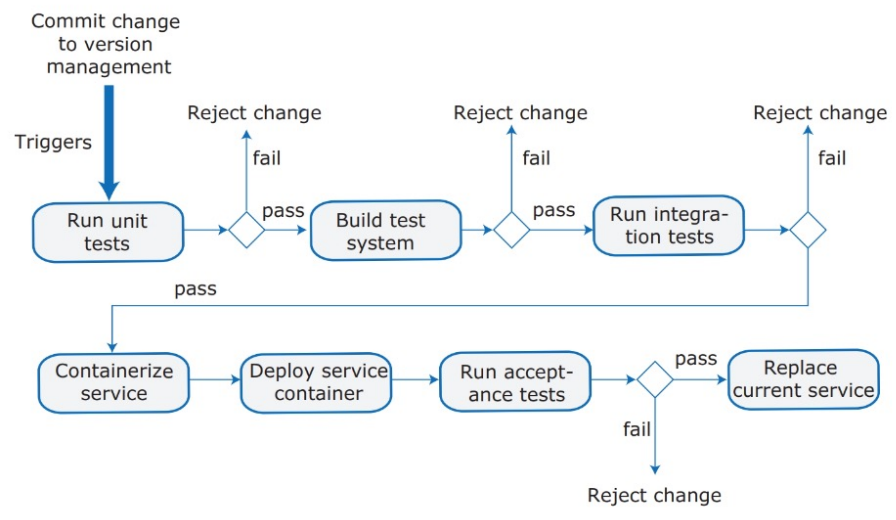
\includegraphics[width=0.93\linewidth,height=0.45\textheight,keepaspectratio]{images/06-microservizi_fig6-8_pipeline-deploy.png}
\caption{Pipeline di Continuous Deployment.}
\end{figure}

La nuova era dell'ingegneria del software è il \textbf{DevOps} (da
\emph{development} + \emph{operations}): \textbf{lo stesso team} si
occupa di sviluppo, deploy e gestione del servizio. La Fig. 6.8 mostra
la pipeline che parte quando c'è un commit: test di unità, build, test
di integrazione, creazione del container, deploy, test di accettazione
e, se tutto va bene, sostituzione del servizio attuale con la nuova
versione.

\subsection{Monitoraggio}\label{monitoraggio}

I test non possono prevenire il 100\% dei problemi imprevisti, quindi
bisogna \textbf{monitorare} i servizi in produzione. Senza monitoraggio
non si conosce lo stato dei servizi, ma un monitoraggio eccessivo
peggiora le prestazioni: come spesso accade con i microservizi, serve un
compromesso.

\begin{figure}[H]
\centering
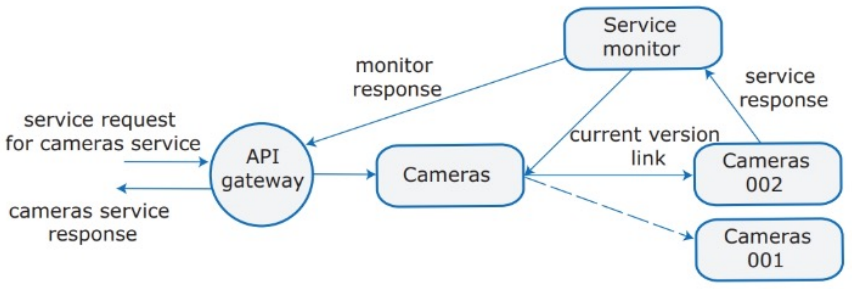
\includegraphics[width=0.88\linewidth,height=0.45\textheight,keepaspectratio]{images/06-microservizi_fig6-9_monitoraggio.png}
\caption{Esempio di monitoraggio.}
\end{figure}

Il monitoraggio aiuta anche l'affidabilità (Fig. 6.9): quando si
introduce una nuova versione di un servizio si può tenere attiva quella
vecchia e spostare il ``\textbf{current version link}'' sulla nuova. Se
il monitoraggio rileva un problema nella nuova versione ``Cameras 002'',
il link torna alla versione 001 del servizio.

\section{Architectural smell}\label{architectural-smell}

\begin{boxdefinition}{Architectural smell}

Un \textbf{architectural smell} è una decisione architetturale di uso
comune che però \textbf{peggiora le qualità} del sistema durante il suo
ciclo di vita.

\end{boxdefinition}

Definiti i principi dei microservizi, come si rilevano gli smell che li
violano e come si risolvono tramite \textbf{refactoring}? Questa sezione
presenta, sulla base di una \emph{multivocal review} (una rassegna che
usa sia articoli scientifici sia siti tecnici), gli smell più
riconosciuti per i microservizi e i refactoring per eliminarli.

I principi di design considerati sono:

\begin{itemize}
\tightlist
\item
  \textbf{Deploy indipendente} (\emph{independent deployability}): ogni
  microservizio deve essere installabile in modo indipendente.
\item
  \textbf{Scalabilità orizzontale} (\emph{horizontal scalability}): ogni
  microservizio deve poter essere scalato in orizzontale, cioè si devono
  poter aggiungere o togliere sue repliche.
\item
  \textbf{Isolamento dei guasti} (\emph{isolation of failures}): i
  guasti devono restare isolati, evitando l'effetto a cascata.
\item
  \textbf{Decentralizzazione} (\emph{decentralization}): va applicata in
  tutti gli aspetti, dalla gestione dei dati alla governance.
\end{itemize}

\subsection{Smell e refactoring}\label{smell-e-refactoring}

Gli smell sono raggruppati per principio violato; per ognuno vediamo i
refactoring che lo risolvono.

\subsubsection{Deploy indipendente}\label{deploy-indipendente}

\begin{itemize}
\tightlist
\item
  \textbf{Smell: più servizi in un container} (\emph{multiple services
  in one container}). Idealmente si vuole un container per
  microservizio. Si può mettere nello stesso container qualche
  microservizio che interagisce molto, ma può creare vari problemi.
\item
  \textbf{Refactoring}: mettere \textbf{ogni servizio in un container
  separato}.
\end{itemize}

\subsubsection{Scalabilità
orizzontale}\label{scalabilituxe0-orizzontale}

\begin{itemize}
\tightlist
\item
  \textbf{Smell: interazione basata su endpoint} (\emph{endpoint-based
  service interaction}). Se si interagisce con \textbf{una specifica
  istanza} di un servizio (Fig. 6.10), aggiungere repliche non fa
  scalare l'applicazione, perché si parla sempre con la stessa replica.
\item
  \textbf{Refactoring}:

  \begin{itemize}
  \tightlist
  \item
    aggiungere un \textbf{service discovery} che dice a chi chiama quale
    replica usare (usato nel 55\% dei casi);
  \item
    aggiungere un \textbf{message router} che inoltra la richiesta a una
    delle repliche, es. un load balancer (31\%);
  \item
    aggiungere un \textbf{message broker} che raccoglie le richieste,
    poi elaborate dalle repliche, es. una coda di messaggi (14\%). È il
    meno usato perché richiede di modificare il codice del
    microservizio.
  \end{itemize}
\end{itemize}

\begin{figure}[H]
\centering
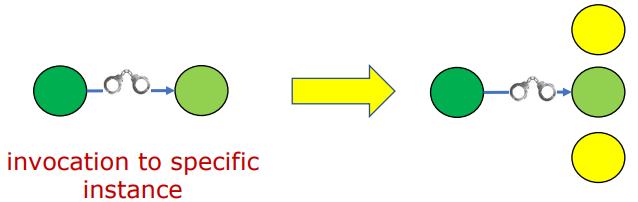
\includegraphics[width=0.65\linewidth,height=0.45\textheight,keepaspectratio]{images/06-microservizi_fig6-10_endpoint-based.png}
\caption{Interazione basata su endpoint.}
\end{figure}

\begin{itemize}
\tightlist
\item
  \textbf{Smell: assenza di un API gateway}: i client chiamano
  direttamente i servizi (simile allo smell precedente).
\item
  \textbf{Refactoring}: aggiungere un \textbf{API gateway}, che oltre a
  risolvere lo smell è utile anche per autenticazione, limitazione del
  traffico (\emph{throttling}), ecc.
\end{itemize}

\subsubsection{Isolamento dei guasti}\label{isolamento-dei-guasti}

\begin{itemize}
\tightlist
\item
  \textbf{Smell: interazione instabile} (\emph{wobbly service
  interaction}): l'interazione di m1 con m2 è ``instabile'' quando un
  guasto di m2 può causare un guasto di m1.
\item
  \textbf{Refactoring}: aggiungere un \textbf{circuit breaker} (42\% dei
  casi), usare dei \textbf{timeout} (22\%), aggiungere un
  \textbf{bulkhead} (20\%) o un \textbf{message broker} (16\%).
\end{itemize}

\begin{boxtip}{Cos'è un bulkhead}

Il nome viene dalle paratie stagne delle navi: si dividono le risorse
(thread, connessioni, \ldots) in compartimenti separati, così se una
parte si blocca non trascina con sé tutto il resto.

\end{boxtip}

\subsubsection{Decentralizzazione}\label{decentralizzazione}

\begin{itemize}
\tightlist
\item
  \textbf{Smell: persistenza condivisa} (\emph{shared persistence}): più
  servizi usano lo stesso database.
\item
  \textbf{Refactoring} (Fig. 6.11):

  \begin{itemize}
  \tightlist
  \item
    \textbf{dividere il database} (50\% dei casi);
  \item
    aggiungere un \textbf{data manager} che fa da gateway tra i servizi
    e il database (22\%);
  \item
    \textbf{unire i servizi} (9\%).
  \end{itemize}
\end{itemize}

\begin{figure}[H]
\centering
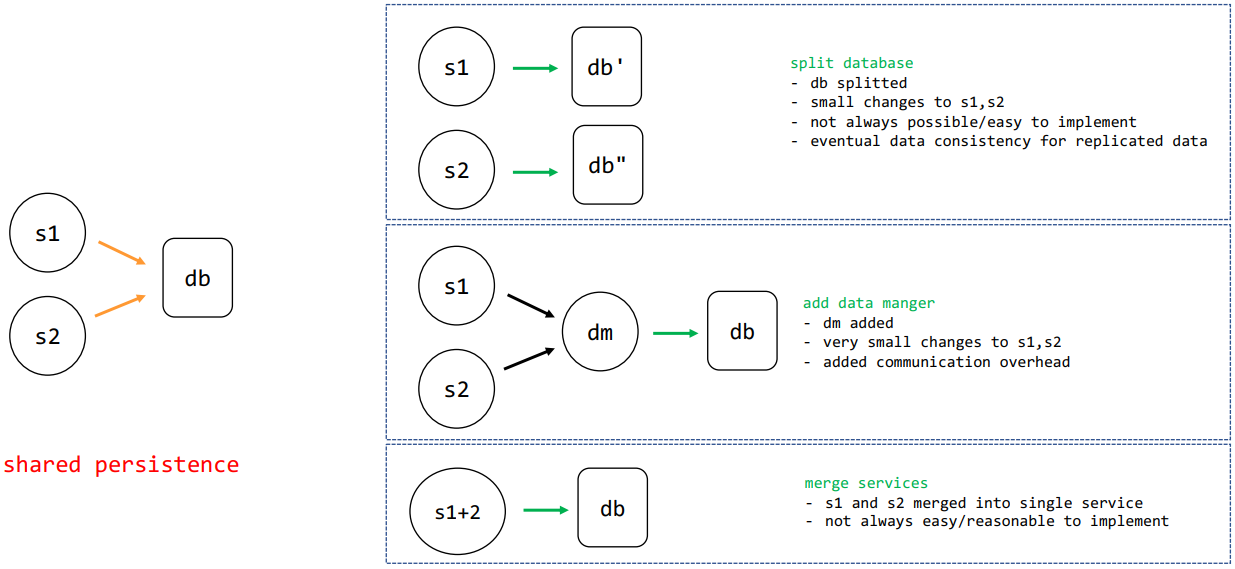
\includegraphics[width=1.00\linewidth,height=0.45\textheight,keepaspectratio]{images/06-microservizi_fig6-11_shared-persistence.png}
\caption{Soluzioni per la persistenza condivisa.}
\end{figure}

\begin{itemize}
\tightlist
\item
  \textbf{Smell: team a livello unico} (\emph{single-layer teams}): team
  divisi per livello tecnico (es. team del database, team
  dell'interfaccia) invece che per servizio. Va contro l'idea di Agile.
\item
  \textbf{Refactoring}: \textbf{dividere i team per servizio}.
\end{itemize}

\subsection{Una toolchain per i
microservizi}\label{una-toolchain-per-i-microservizi}

Ora che conosciamo gli smell, vogliamo trovarli e risolverli. Il primo
passo è creare una \textbf{rappresentazione grafica} dell'architettura
(Fig. 6.12), per capire meglio la struttura dell'applicazione.

Questi modelli permettono anche \textbf{viste per team}, visto che ogni
servizio è sviluppato da un team diverso. È utile soprattutto quando ci
sono smell tra microservizi gestiti da team diversi: i team possono
accorgersene e mettersi d'accordo per risolverli.

\begin{figure}[H]
\centering
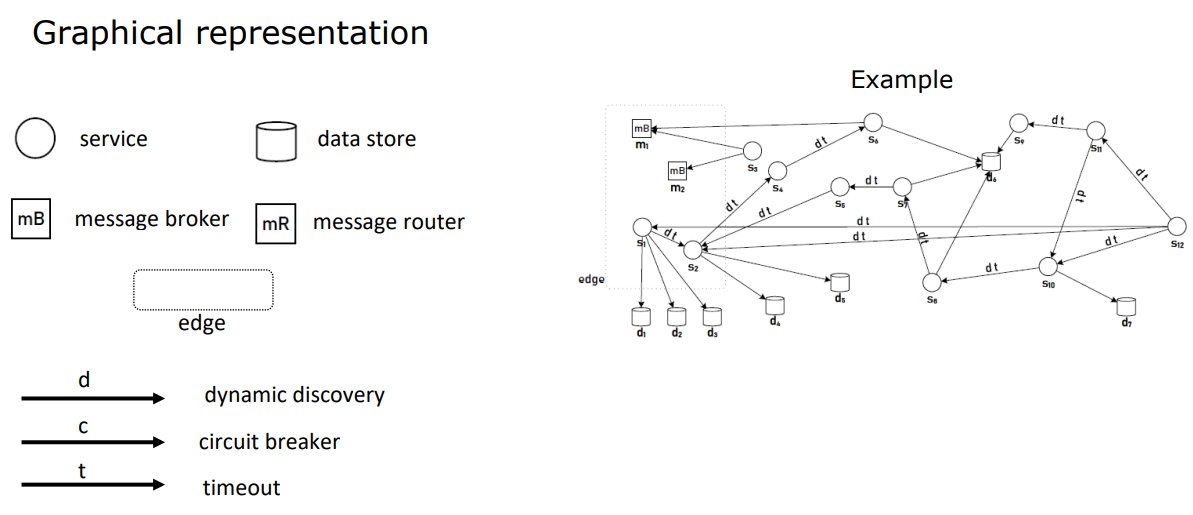
\includegraphics[width=1.00\linewidth,height=0.45\textheight,keepaspectratio]{images/06-microservizi_fig6-12_modello-architettura.png}
\caption{Modellare l'architettura di un'applicazione.}
\end{figure}

Esistono strumenti che ricevono questi modelli e restituiscono gli smell
presenti. Uno è stato sviluppato all'Università di Pisa:
\textbf{MicroFreshener}
(\href{https://github.com/di-unipi-socc/microFreshener}{GitHub}). Per
sistemi grandi può essere difficile ottenere a mano il modello
dell'architettura, quindi sono stati creati strumenti
(\textbf{MicroMiner} e \textbf{MicroTOM}) che lo ricavano analizzando i
manifest K8s e facendo analisi dinamica dell'applicazione in esecuzione
(l'orchestrazione dei container, infatti, cambia il comportamento
dell'applicazione). La Fig. 6.13 mostra la toolchain completa.

\begin{figure}[H]
\centering
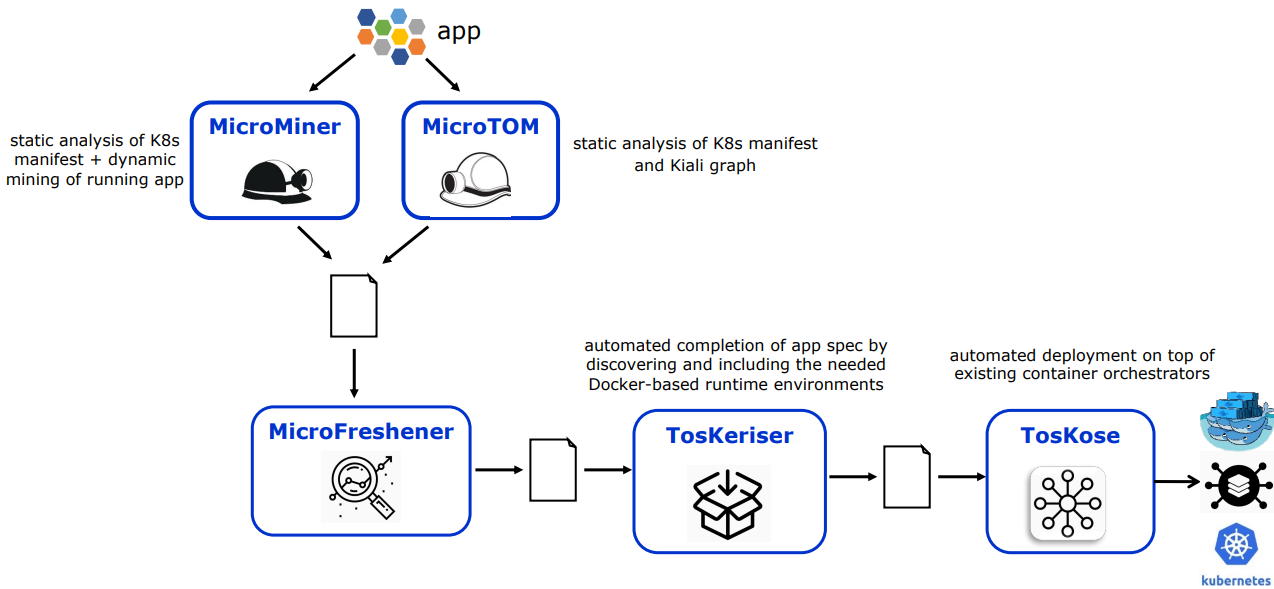
\includegraphics[width=1.00\linewidth,height=0.45\textheight,keepaspectratio]{images/06-microservizi_fig6-13_toolchain.png}
\caption{Toolchain per i microservizi.}
\end{figure}

Dopo aver analizzato gli smell e applicato le correzioni in
MicroFreshener, il risultato si può \textbf{installare automaticamente}
sull'orchestratore di container già esistente (nella toolchain, con
TosKeriser e TosKose).
